\documentclass[12pt,a4]{article}
% \usepackage{draftwatermark}
\usepackage{background}
\usepackage{color}   %May be necessary if you want to color links
\usepackage{hyperref}
\hypersetup{
    colorlinks=true, %set true if you want colored links
    linktoc=all,     %set to all if you want both sections and subsections linked
    linkcolor=blue,  %choose some color if you want links to stand out
}
\textwidth 170 mm
\oddsidemargin -8 mm
\evensidemargin -8 mm
%\SetWatermarkScale{3.0}
\SetBgColor{red}
\SetBgOpacity{0.1}
\SetBgScale{10}
%\SetBgContents{\hspace{9mm} \hspace{0mm}\vspace{2mm} \includegraphics[width=5mm]{Alfresco_logo_CMYK_white}} 

\begin{document}
\begin{center}
{\Large Capacity planning: estimate the disk space used by indexes}

\vspace{5mm}

\Large{Solr vs Lucene}

\vspace{5mm}
{\bf Alex Madon}
\vspace{5mm}

\today

\vspace{15mm}
% {\huge To be reviewed}

\end{center}
\vspace{5mm}

\newpage

\tableofcontents

\newpage

\section{Introduction}
Customers are sometimes interested in evaluating the space used to store the indexes when the space used by the documents is known in advance.

When doing capacity planning, there are generally two methods\cite{allspaw}
: one is to experiment and then extrapolate the experimental rules observed; the second is to compute the space used based on the space bits of information theoretically use. One example of the second approach is the capacity planning formula used to describe the memory needed by Solr as a function of the N = number of Nodes in store
T = number of transactions in repo
A = number of ACLs in repo
X = number of acl transactions in repo
https://issues.alfresco.com/jira/browse/MNT-1937

In this article, we will use the 2nd method to estimate the space needed to store the indexes.



\section{What we are looking for}
Customers usually have an accurate estimation of the volume of data they plan to inject into alfresco.
They will probably know the number (N) of documents to upload, as well as the average size of the documents.

Often the directory storing the file (the alf\_data folder) will be on one partition, and the indexes will be stored on another partition. This difference in storage could be caused because lucene indexes have to be local to the machine, and data file can reside remotely. In the case of solr, this could simply be because the solr machine is different form the alfresco node.

We are looking for the ratio

\begin{equation}
R=\frac{index\_size}{data\_size}
\end{equation}
where $index\_size$ is the size of the index and $data\_size$ is the size of the data (as in alf\_data.

If the index size grows linearly (as a first approximation) with the data size, then we can use the our few measure of R to evaluate the size of the indexes.

\section{A general methodology}
A general method to get an estimate of the ratio, would be to generate a corpus of 'typical' documents that would be used.
Then you get X amount of those documents, and you measure the ratio R.
Then you multiply X by 2 (or some other factor) and you measure the new R.
You confirm then that the index size grows linearly with the data size and are thus able to evaluate the storage space needed to sore the indexes.

\section{Our methodology}
In this article we cannot define typical documents, as a document will be typical only to a given customer.
To get useful result we use a corpus of document with well known and defined properties.
Those properties are detailed in the next sections.

Note that we could have chosen corpus available on the Internet. We commonly used corpus when it comes to indexing performance is the Wikipedia data. Indeed, Wikipedia pages can be downloaded from the internet at http://dumps.wikimedia.org/




\section{Finding out what the ratio depends on}
Indexes used in alfresco are mainly inverted indexes: each token seen in the documents will point to a list of documents containing the token and the position of the token within the document.

\subsection{The model}
Alfresco allows to define custom models.
An extreme case would be to create a model that contains zero data and only meta-data.
In that case, we would have a very large ratio R.
From now on, we suppose that there is no other meta data that the default meta-data when using the default (out of the box) model, where no specific metadata is inserted (as description or title). The only metadata known is the time of the upload, owner of the document and document name.
 
\subsection{The MIME type of the content}

A huge dependency will be on the amount of text a given file type can contain.
For instance a video file is a binary file that contains mainly binary video, and very few txt (maybe just few meta data).
On the other hand a text file will only contain text file.
To index data, alfresco will first transform to text the documents that are uploaded to it.
In the case of video files, we would thus expect that the ration is much smaller than in the case with text.

\subsubsection{PDF}
To illustrate this, let's create a PDF file containing just two words. Let's then convert it to text (using pdftotext for instance) and look at the sizes of the PDF and TXT versions:

\begin{verbatim}
-rw-r--r-- 1 madon madon 9157 Apr 29 14:45 test.pdf
-rw-r--r-- 1 madon madon   10 Apr 29 14:47 test.txt
\end{verbatim}

\begin{verbatim}
wc test.txt
 4  2 10 test.txt
\end{verbatim}
It has 4 lines and 2 words and 10 bytes.
9157/10=915 times more space

\subsubsection{Office 2007}
Similarly, a Office 2007 Word document containing just one word ('alex') will be much larger than the text version.
\begin{verbatim}
ls -l test1.docx
-rw-r--r-- 1 madon madon 3792 Apr 29 14:51 test1.docx
\end{verbatim}
one word 'alex' (4 bytes)
3792/4=948

\subsubsection{TXT: our worst case scenario}
The customer has thus to do some work and try to identify what would be the typical data to upload.
This may be difficult sometimes, as customers use a mix of mime types: videos, PDF, Office files, etc...

What could be the rule we communicate to customers to help them in their capacity planning.
What would be useful is instead of answering the very general question

``what is the space used by lucene as a function the the space used by the data''

we answer the following question:


``what is the space used by lucene as a function the the space used by the data in the worst case scenario?''

That would give the customers an {\bf upper bound} of the space used by the indexes.
From now on, we will limit ourselves to the study of the the size of the indexes when all the content is Text.


Note: we have assumed that the TXT format is the format that contains the most amount of the text information.
We exclude compressed text. If you use a log of compressed data (gzip, zip, compress, etc...), you do want to check that your mime type respects the the above rule, that is that the size of the extracted text is larger than the size of the original document uploaded to Alfresco.

\subsection{The vocabulary or number of possible tokens}

The entries of the index depends on the number of tokens.
The number of tokens depends on the language used or vocabulary used.
For instance, some language like Chinese have a very large number of unique words around 20000 words.
Other languages have a more restricted vocabulary; Stemming can also be used to reduce the number of tokens.
For instance when the indexer finds the word 'singing' in a document, it will index the stem 'sing-'.
You can also have an installation where documents are in different languages: English, French, German, Chinese, Japanese, Korean, Thai, etc...
In this article, we do explorer this dimension of parameters. We however simplify the mechanism and we create our own model of vocabulary.
We first create a vocabulary choose W words randomly. The words have a length between 1 and 12.
Note that the method we use allow for duplicate words, and duplication is more likely to happen for short words.

We tested three vocabularies with three different distributions. A vocabulary is an array of words. Then a document is generated picking radomly 10000 words in that array and separating them using a space.
\subsubsection{Vocabulary 1}
The first vocabulary is genertaed following the pseudo-code below:
\begin{verbatim}
words=list()
for i in NUMBER_OF_WORDS:
   len=random(1,12)
   word=''
   for i in range(0,len):
        word=word+random_lower_case_ascii
   words.append(word)
\end{verbatim}
we choose a random length for the word between 1 and 12, and then we build a word choosing random (lowercase ASCII) letters to build a word of that length.
This distribution will probably have duplicate words.
\subsubsection{Vocabulary 2}
The pseudo code is below:
\begin{verbatim}
    words=[]
    for i in range(97,123):
        word=chr(i)
        words.append(word)
        for j in range(97,123):
            word=chr(i)+chr(j)
            words.append(word)
            for k in range(97,123):
                word=chr(i)+chr(j)+chr(k)
                words.append(word)
                for l in range(97,123):
                    word=chr(i)+chr(j)+chr(k)+chr(l)
                    words.append(word)

\end{verbatim}
this ensures there is no duplicate words in the vocabulary array.
It is also the most diverse vocabulary of words of length between 1 and 4 that can be build with lowercase ASCII letters.
\subsubsection{Vocabulary 3}
As the ratio observed with the vocabulary 2 was worse that with vocabulary 1, we created a 3rd vocabulary, then is expected to be even worse; It consists of one letter words build with one unicode character from the digits, ascii, greek, cyrillic, hebrew, arabic, thai and CJK (Chinese Japanese Korean) characters:
\begin{verbatim}
    planes=[
        ('\u0030','\u0039'), # digits
        ('\u0061','\u007A'), # letters
        ('\u03AC','\u03C9'), # greek
        ('\u0430','\u044E'), # cyrillic
        ('\u05D0','\u05EA'), # hebrew
        ('\u0622','\u06D3'), # arabic
        ('\u0E01','\u0E2F'), # thai
        ('\u4E00','\u62FF'), # CJK1
        ('\u6300','\u77FF'), # CJK2
        ('\u7800','\u8CFF'), # CJK3
        ('\u8D00','\u9FFF'), # CJK4
        ]
    for (afrom, ato) in planes:
        for i in range(ord(afrom),ord(ato)+1):
            words.append(chr(i))
\end{verbatim}
This vocabularyu is expecte to generate small text files that will need a relative large index to store the variety of tokens.

\subsection{Stop words}
Using stop words is known to reduce the size of indexes.
In this article we do not use stop words (other than the one defined by default which may happen to be used by our own created vocabulary).
 
\subsection{Document truncation}
The length of the document is also a possible candidate parameter to explore. In this article we do not explorer it. We create special documents which all contain 10000 characters. This correspond to lucene.indexer.maxFieldLength. Alfresco ignores words that come after that amount of words in the document.



\section{Our document model}
From the section above, we can summarize the properties of the documents we we use.

The documents will be created choose 10000 words randomly in a vocabulary V.
The vocabulary is itself composed by a number W of words (token). Those tokens are randomly chose a chains of n lowercase alphabetic characters where n is a random number between 1 and 12 .

Those documents are then upload to Alfresco 4.1.3 using the REST upload API.

The number of documents we upload is 1000. We could have investigated this parameter also but due to lack of resources and because the ratio seemed to behave linearly, we did not vary this parameter.

We looked at both index subsystems: lucene and solr.

After each test (new index subsystem or new vocabulary), a new alfresco was created


The table shows the results as the index subsystem changes and the vocabulary changes.

\section{Results}
\subsection{Ratio as a function of the indexing subsystem and number of words in the vocabulary}
\begin{table}[h]
\begin{center}
\begin{tabular}{|c | r | c|}
\hline
index & W = words in vocab. & R = Index/Data\\ \hline
lucene & 100 & 18\%\\
lucene & 5000 & 34\%\\
lucene & 20000 & 37\%\\
solr & 100 & 10\%\\
solr & 5000 & 62\%\\
solr & 20000 & 70\%\\
solr & 300000 & 89\%\\
\hline
\end{tabular}
\end{center}
\caption{For 1000 docs}
\end{table}

\subsection{Ratio as a function of number of documents}
The ratio is relatively stable as a function of the number of documents as shown by the table below.
\begin{table}[h]
\begin{center}
\begin{tabular}{|c | r  | r| c|}
\hline
1000 &89512 & 80144 & 89\%\\
2000 &161104 & 158408& 98\%\\
3000 & 231876 & 226116& 98\%\\
5000 & 375620 & 358512 & 95\%\\
\hline
\end{tabular}
\end{center}
\caption{For solr 300k words vocabulary}
\end{table}


\subsection{Ratio as a function of time and vocabulary}
A VIDEO for solr with 300k words in vocabulary and 5000 docs

http://madon.net/video\_solr\_noaudio.mp4


\begin{figure}[h]
\begin{center}
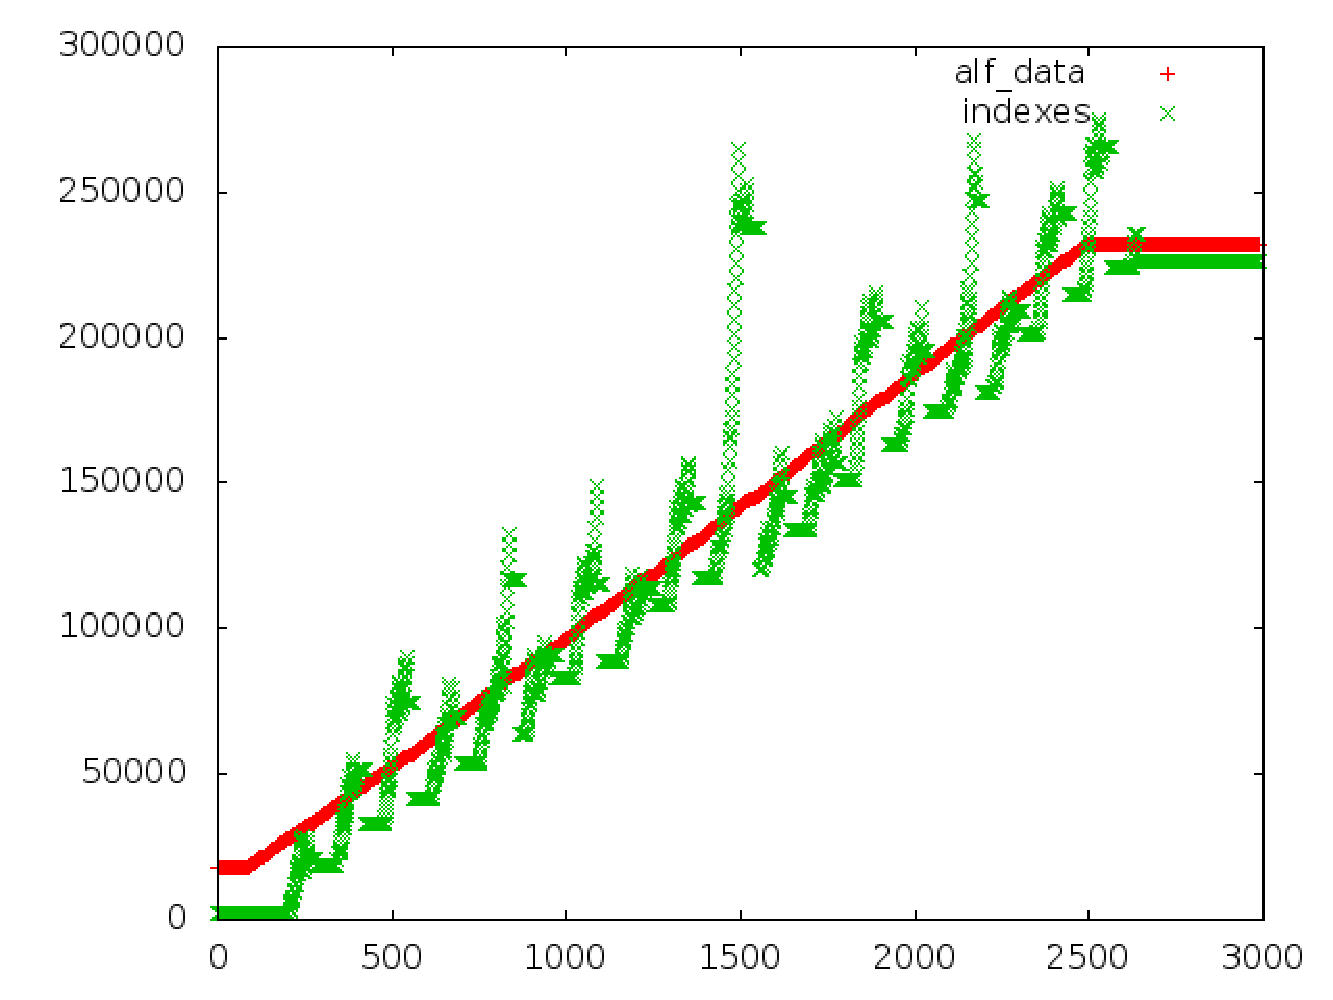
\includegraphics[width=130mm]{solr_3kdocs_300kwords}
\end{center}
\caption{Vocabulary 1: Comparison of the disk space used by the data (in red) with the disk space used by the solr indexes (in green) while uploading 3k documents with a 300k words vocabulary. The horizontal axis is the time in 10th or seconds, the vertical axis is the disk used in bytes.}
\end{figure}



\begin{figure}[h]
\begin{center}
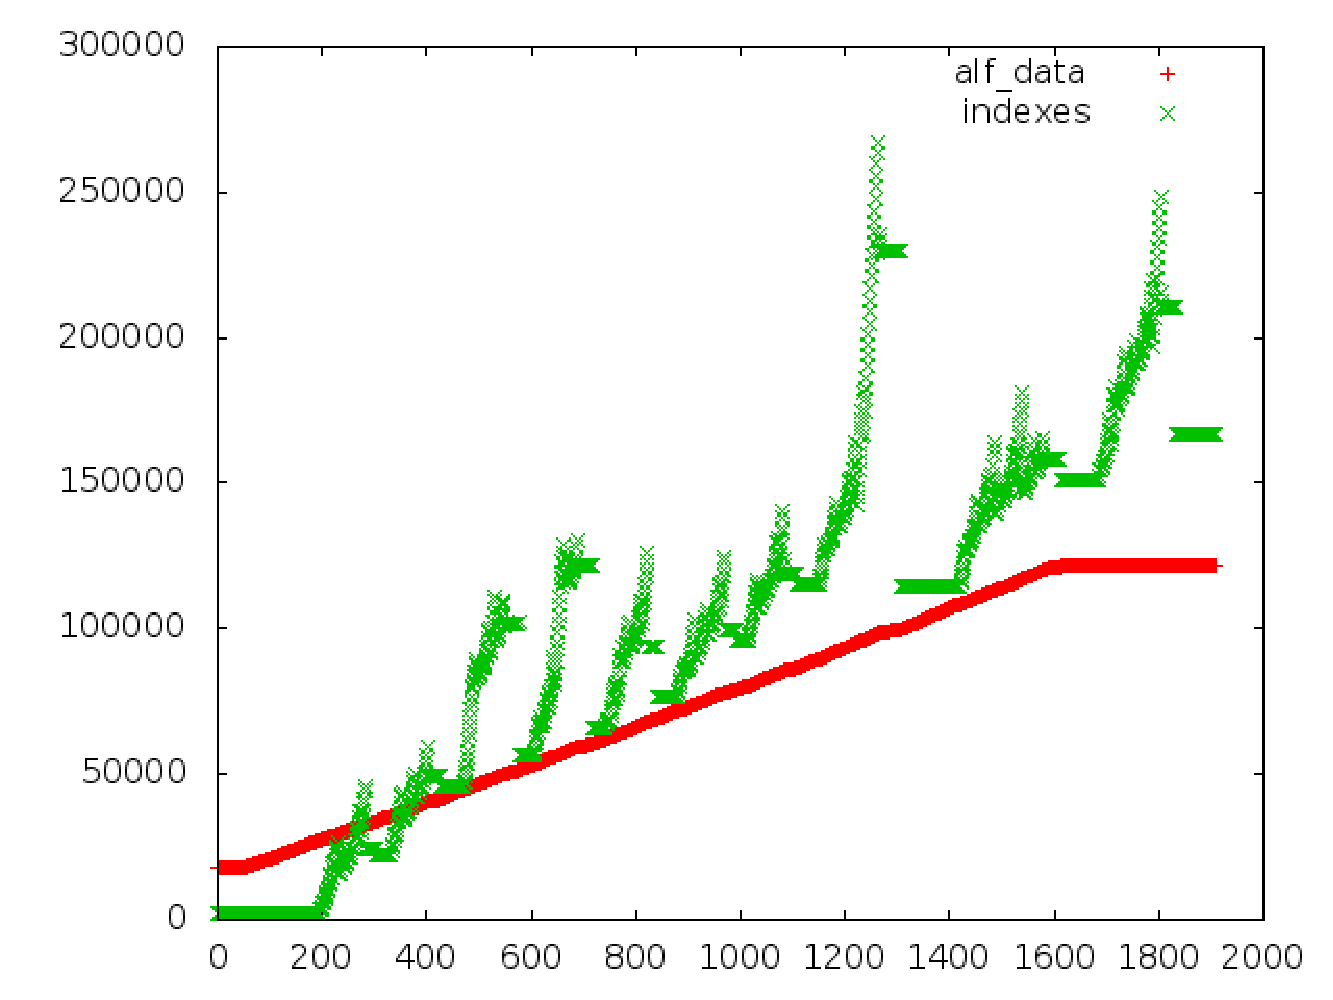
\includegraphics[width=130mm]{out_vocab2_2kdocs}
\end{center}
\caption{Vocabulary 2, 2k docs: Comparison of the disk space used by the data (in red) with the disk space used by the solr indexes (in green) while uploading 2k documents with a 300k words vocabulary.}
\end{figure}


\begin{figure}[h]
\begin{center}
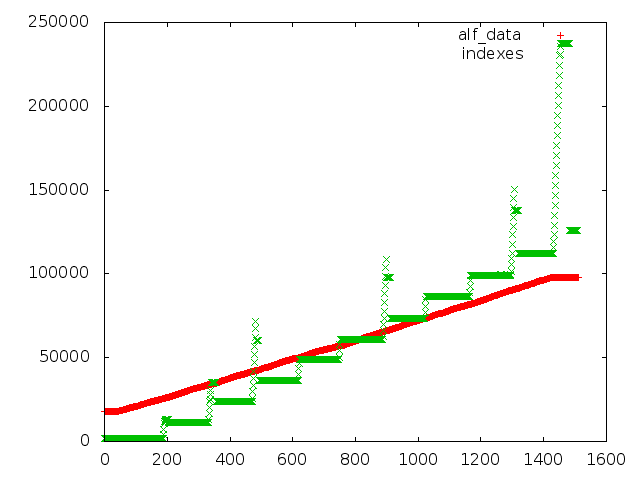
\includegraphics[width=130mm]{out_vocab3_2kdocs}
\end{center}
\caption{Vocabulary 3, 2k docs: Comparison of the disk space used by the data (in red) with the disk space used by the solr indexes (in green) while uploading 2k documents with a UTF8 vocabulary.}
\end{figure}



\begin{figure}[h]
\begin{center}
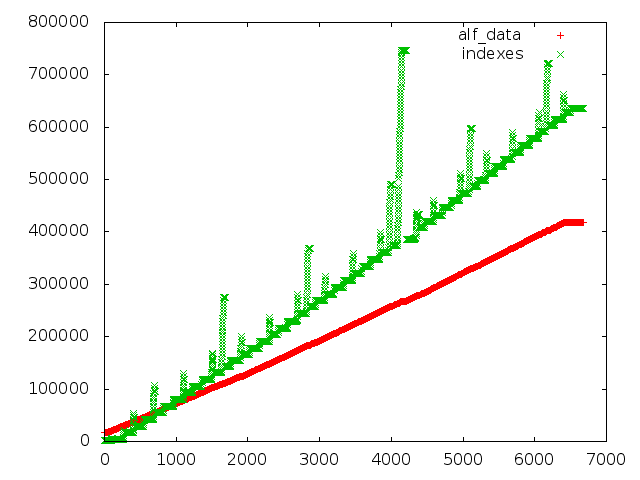
\includegraphics[width=130mm]{out_vocab3_10kdocs}
\end{center}
\caption{Vocabulary3 , 10k docs: Comparison of the disk space used by the data (in red) with the disk space used by the solr indexes (in green) while uploading 3k documents with a UTF8 vocabulary.}
\end{figure}

\begin{figure}[h]
\begin{center}
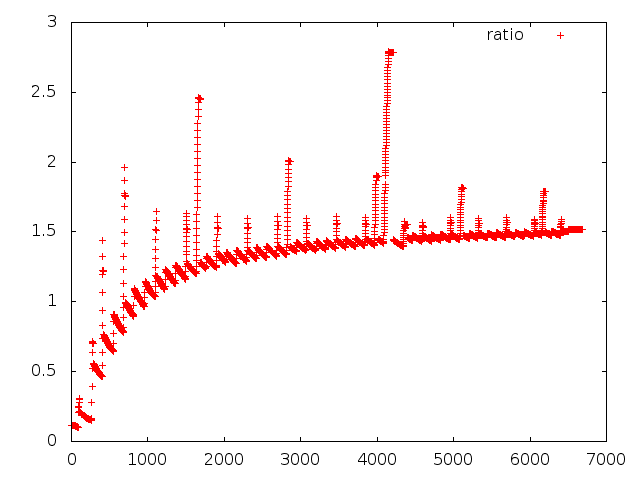
\includegraphics[width=130mm]{out_ratio_vocab3_10k}
\end{center}
\caption{vocab3, 10k words, ratio Comparison of the disk space used by the data (in red) with the disk space used by the solr indexes (in green) while uploading 3k documents with a 300k words vocabulary}
\end{figure}



\section{Analysis}
\section{Ratio as a function of the subsystem used}
Solr indexes take approximately twice the space used by Lucene.
This is because by default solr with index one document twice: one with stemming based on the locale of the document and once without stemming (standard analyzer).
This is done to improve search accuracy when the locale of the search client is different from the locale of the document.
The resulting tokens is then also multiplied by two,.
This can be easily seen in the solr admin page using the luke index analyzer, see screen shot
 
http://localhost:8080/solr/alfresco/admin/luke?wt=xslt\&tr=luke.xsl



\begin{figure}[h]
\begin{center}
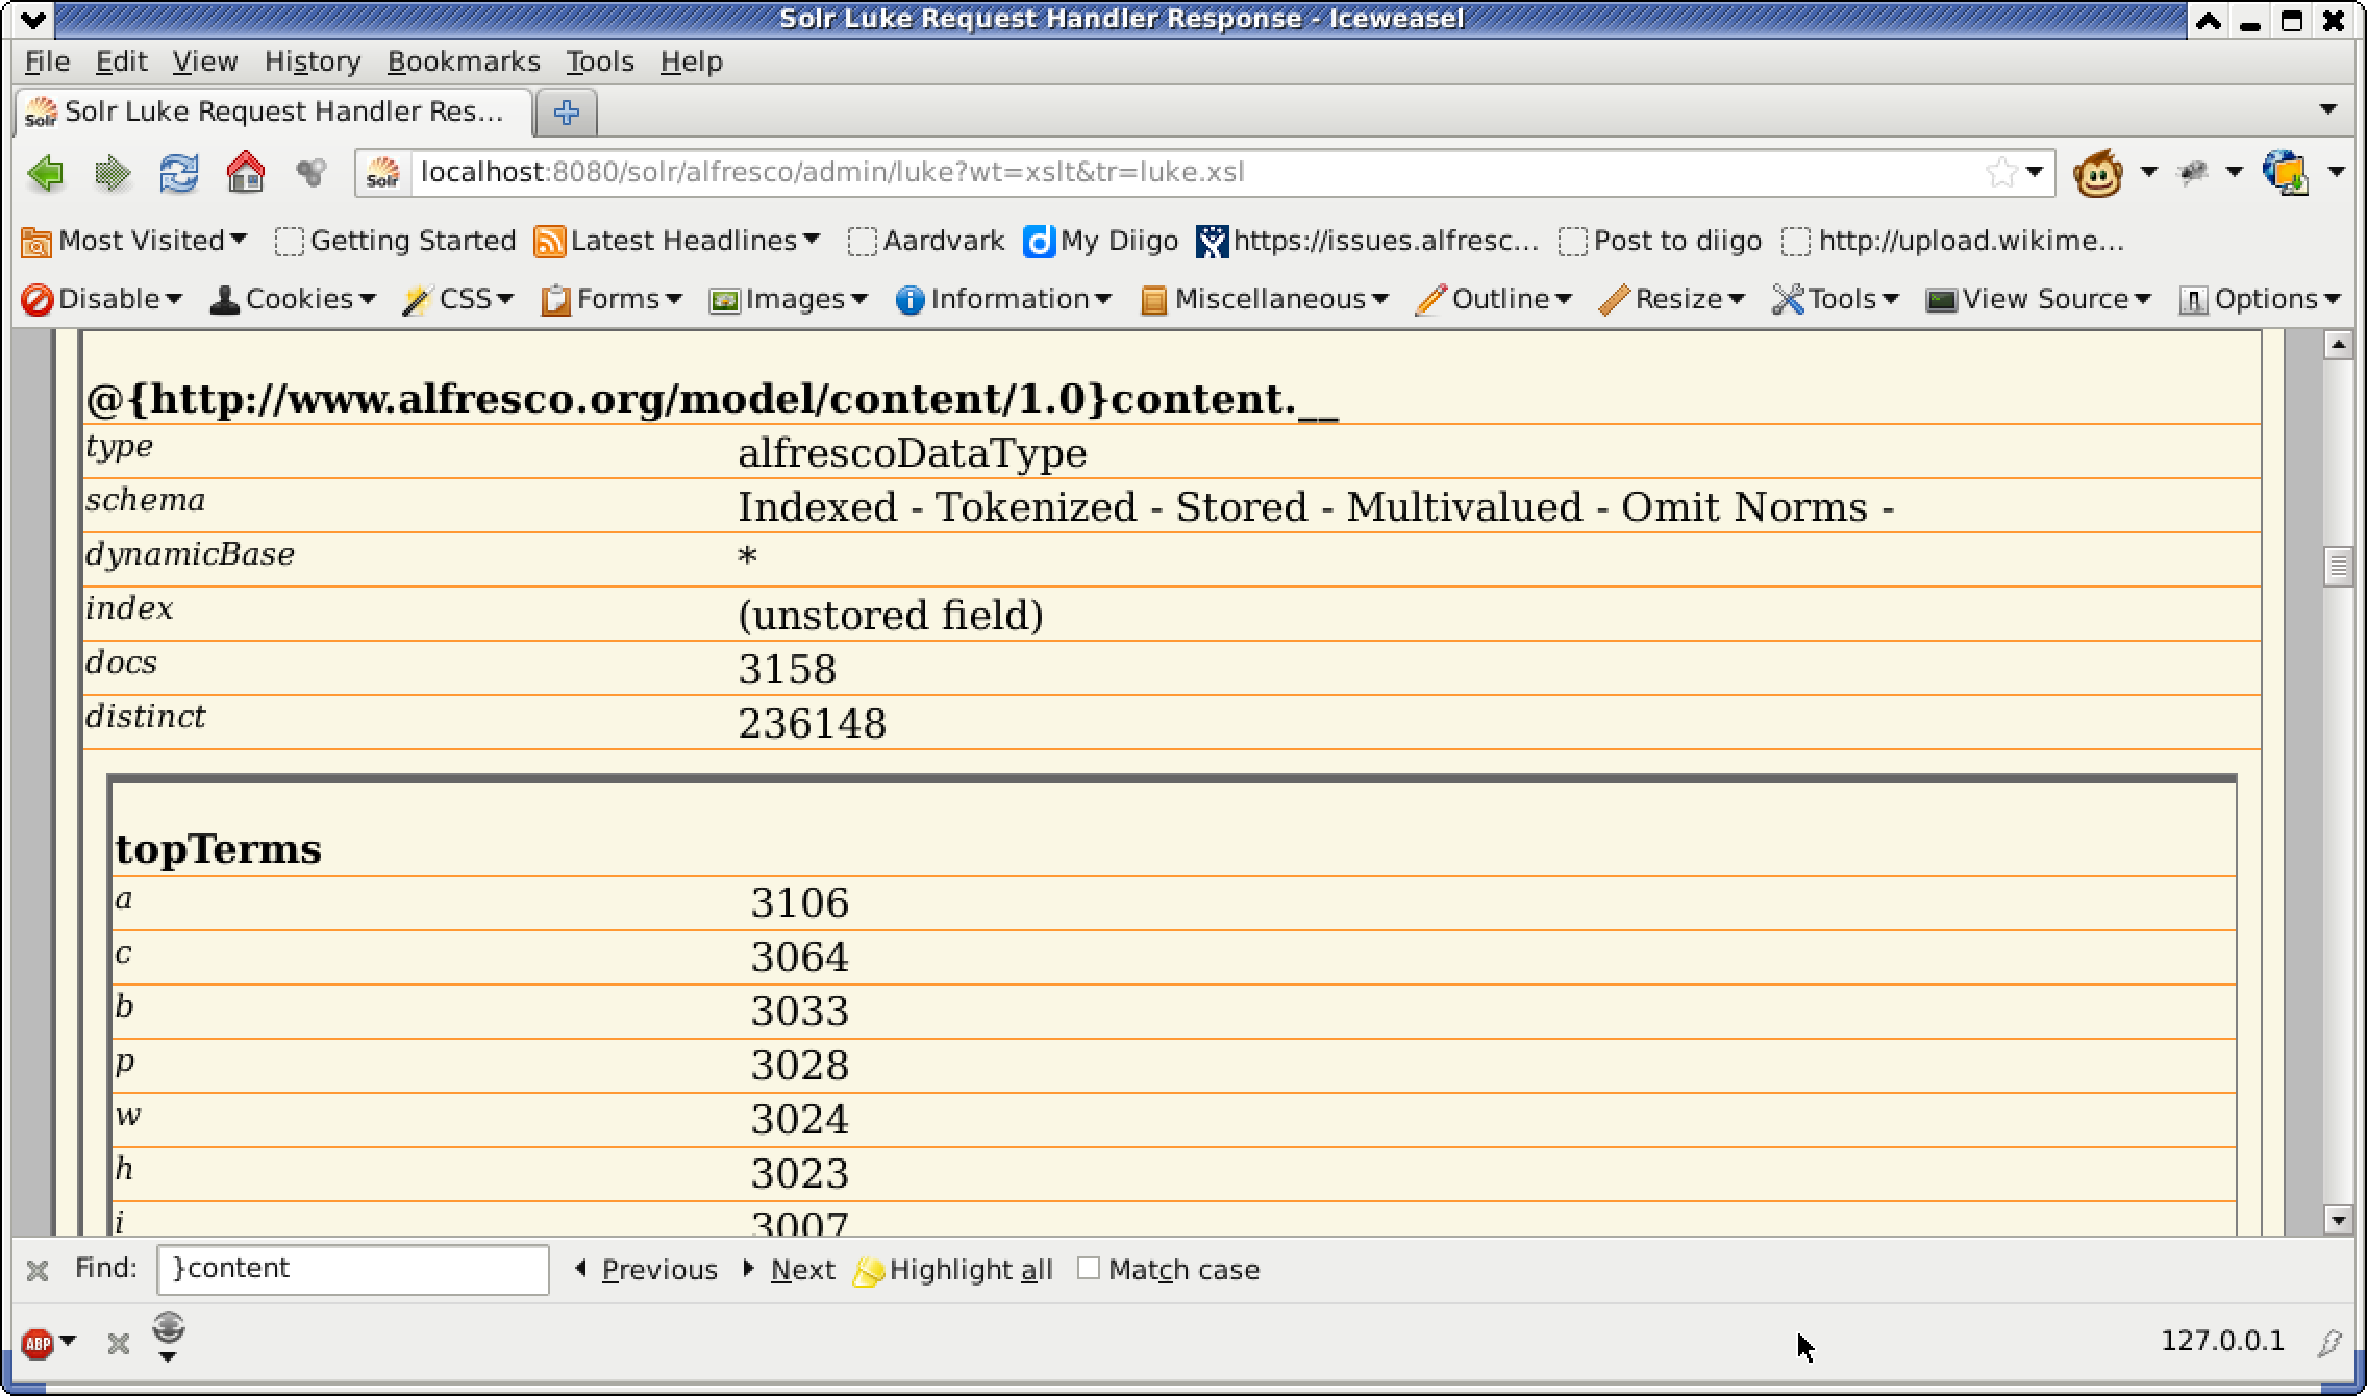
\includegraphics[width=130mm]{luke_content__}
\end{center}
\caption{luke content underscore underscore: the tokens are not marked with the locale.}
\end{figure}



\begin{figure}[h]
\begin{center}
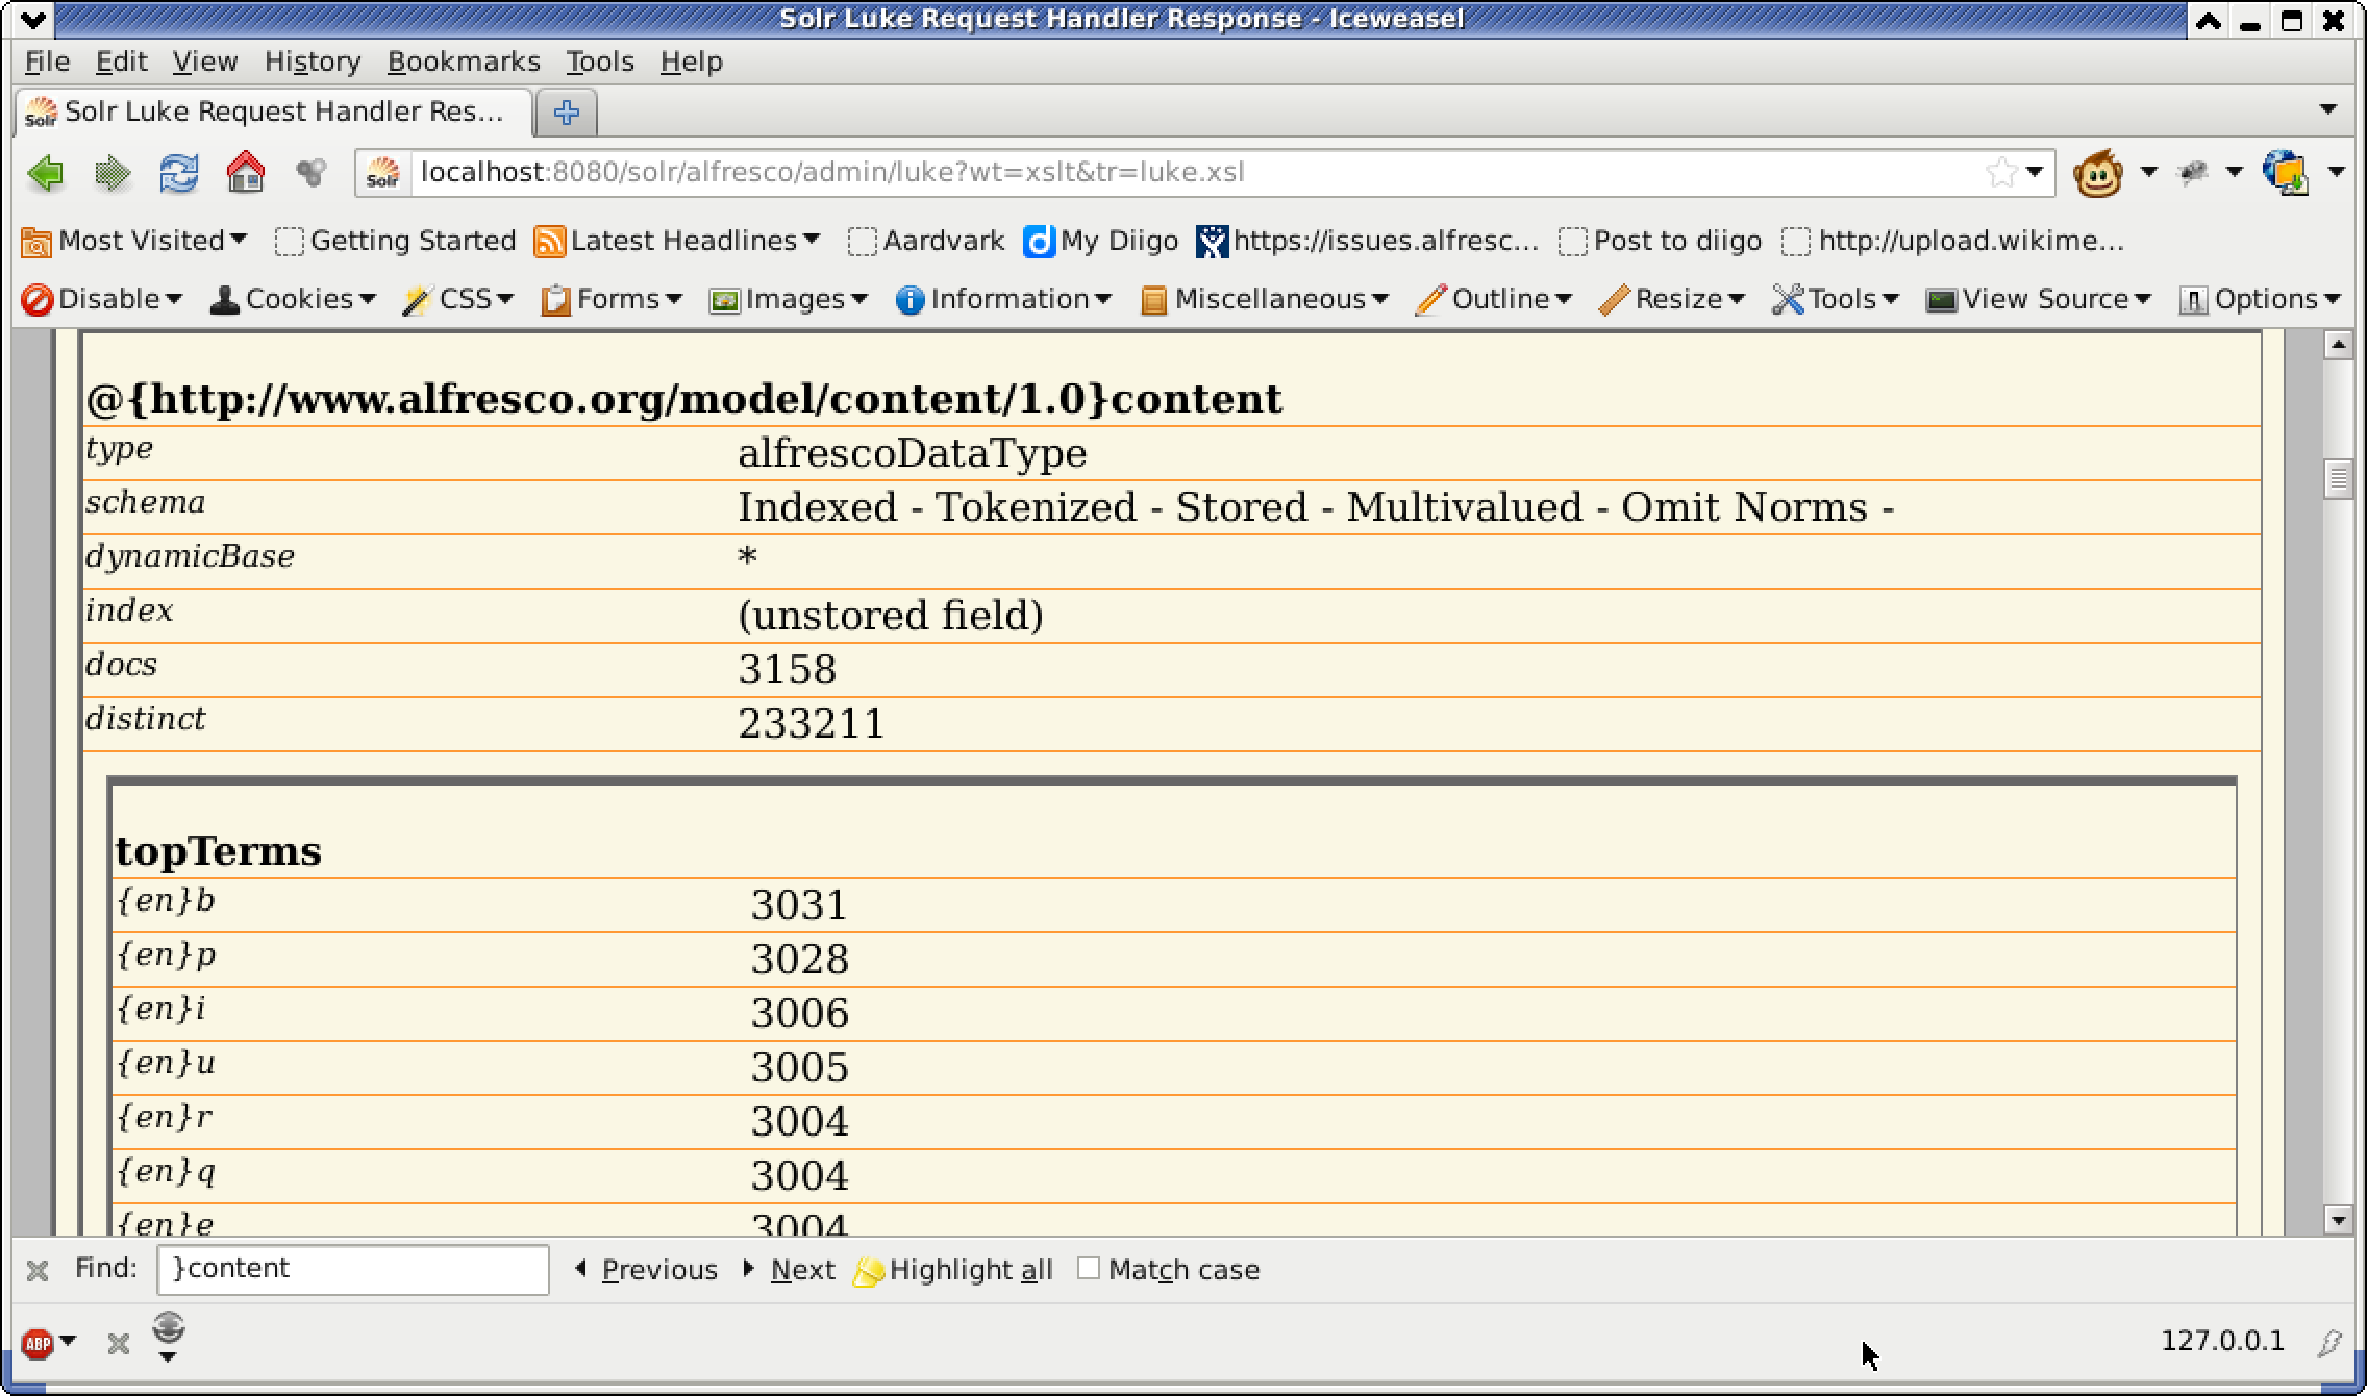
\includegraphics[width=130mm]{luke_content}
\end{center}
\caption{luke content: the tokens are not marked with the locale.}
\end{figure}

\section{Ratio as a function of the number of words in the vocabulary}
The more words you have in the vocabulary, the larger the indexes will be.


\section{Ratio as a function of time}
We observe bursts.
These are caused by index merging.

\section{Note about backups}
alf\_data/backup-lucene-indexes

depending on your configuration see 

http://docs.alfresco.com/4.1/topic/com.alfresco.enterprise.doc/concepts/solr-backup-recovery.html

alf\_data/solrBackup

Note that this is not subject to the burst of disk usage we observe on the live indexes.


\section{Conclusion}

In this article we have used an experimental method to evaluate the disk space used by the indexes. As we understand the ratio depends on the content, we were particularly interested in getting an upper bound value for the ratio of the space used by indexes by the space used by the data.

As indexes allow search, ideally customers would be looking for a small ratio. However, we showed in controlled experiments that the ratio can become high in particular that more space may be needed to store the indexes than the data. But of course that depends on the data.

We fixed the document length to 10000 words as Alfresco by default will not index the content after the 10000th word.

We restricted ourselves to the case where the document mime type was text/plain: indeed the worst case for the ratio will be with text document: Alfresco always extracts the text from the documents and text is the most efficient format (uncompressed) to store the information that we know.

We then investigated dependency on the number of documents. The larger the number of documents, the larger the indexes, but the increase is slow.

We investigated depending on the index subsystem: solr uses approximately twice the space needed by lucene; This is due to a design choice that aims at accurate search in multi locale environments.

We investigate depending time.
Merging of indexes can require up to twice the amount of a stable index (where no document is added or modified).

We also investigated depending on the vocabulary. Vocabularies with a lot of different small words (like the ones used with oriental Characters like Chinese) tend to need much more space with a ration reaching 1.3 (or 130\%). With bursts doubling the size of the index during short periods of time, the ration because 2.6 (or 260\%). As you always want to avoid a disk full on the indexer, you need also to add a safety margin.

For vocabularies based on ASCII characters, the ratio with solr is more typically around .4 (40\%). With the index merging phenomena plus the margin that has to be multiplied by at least 2.

Finally, both lucene and solr, a backup of the index occurs. This multiplies also the disk space usage by two, however, there is no burst phenomenon with the backup folder.

Finally, it may be that the customer's data is far for the scenario we presented here. Indeed when creating those scenarii, in particular when looking at the vocabulary to use, we were trying to create the worst case scenario.
The customer is thus invited to do the experiments himself, using sample of real data. Alternatively, Alfresco Consultants could also be hired to get more accurate pictures.


\begin{thebibliography}{9}

\bibitem{allspaw}
{\bf The Art of Capacity Planning: Scaling Web Resources: Being Ready for the Big Growth Spurt}, by John Allspaw (30 Sep 2008)
O'Reilly, 156 pages
 \end{thebibliography}


\end{document}
